\documentclass[authoryear, 12pt,5p, times]{elsarticle}
\usepackage[hypcap]{caption}
\usepackage{float}
\usepackage{amsmath}
\usepackage[hidelinks]{hyperref} 
 \usepackage{gensymb}
\usepackage{subcaption}
\usepackage{url}
%\renewcommand\thefootnote{\fnsymbol{\dagger}}
\usepackage[symbol*]{footmisc}
\begin{document}
%\footnote{This is a footnote}
\begin{frontmatter}
\title{Astronomical Spectroscopy: Detecting light with a CCD}
\author{\today \\ \quad \\Jung Lin (Doris) Lee\\ dorislee@berkeley.edu\\Group partners: Jennifer Ito, Manuel Silvia\\Prof. James Graham, UGSI Heechan Yuk, Isaac Domagalski}
	\begin{abstract}
    %key objective, method, principle conclusion 
	ABSTRACT HERE
	Spectroscopy is a essential tool in observational astronomy for examining  properties of astronomical bodies. In this experiment, we observe the different spectral line signatures of different everyday light sources. Systematic effect due to (1),(2), and (3), the main ones we correct for are (2),(3). We find that the  $---$ closely match with Poisson error. The smoothing of data serves to improve the accuracy of the centroid-finding algorithm as it eliminates tiny differences to be indentified as improtant signature. However, the automated centroid-finding algorithm that we employed was still not on par with the results obtained by visual estimation of data range cutoffs. Therefore, using these centroid values, we fit a third-order polynomial using the least squares method and obtained parameter $----$\% close to the manifacturer's equation for wavelength calibration.
  
	\end{abstract}
\end{frontmatter}
\section{Introduction\label{intro}}
Optical spectroscopy provides important information about the chemical composition observational targets as, in most cases, astronomers do not have access to physical samples of their targets for conducting detailed chemical analysis. Detailed insight into the properties of planetary bodies, radiating black-bodies, and their  surrounding medium can be derived from atomic absorption and emission lines features on a spectra.
Early models of spectrometers consist of prisms that $----$ . However, most modern day spectroscope uses finely-grated slits instead of prisims to minimize absorption so that faint sources (common to astronomical observation) can be better observed. Moreover, the use of optical fiber plates for multiple spectra to be taken simultaneously enables cosmological studies such as Baryon Oscillation Spectroscopic Survey (BOSS; Dawson et al.) to examine higher redshift targets quasars and luminous red galaxies.

A spectroscope is an arrangement of instrument used for $----$.  It consist of a series of $----$. The incoming light is collimated and goes through the diffraction grating which disperses the beam into component of different wavelengths.  Then the dispersed light is detected by the CCD with side-by-side pixels that span a fixed range of wavelengths. The intensity value incident on each pixel is converted into digital units and read to a computer for further analysis.  Therefore each dispersed component falls into one of the ranges .

In this report, we present the internal workings of a spectrometer and how that effects the raw, unprocessed spectra obtained. In section 2, I will present the Ocean Optics USB 2000 spectrometer hardware used for this experiment and a qualitative overview of the data resulting from different sources. In section 3, I will detail the various procedures that were used to eliminate noise and variations associated with the spectrometer's hardware setup.  Then, section 4 explores the Poisson nature of these systematic effects. Finally, section 5 explains how we converted the pixel values recorded by the spectrometer to the more hardware-independent measure of wavelength by comparing our data with given spectral features  and corresponding wavelengths from NIST\footnote{National Institute of Standards and Technology Atomic Spectra Database}.
\section{Hardware and Experiment}
	\subsection{Ocean Optics USB 2000 spectrometer}
The spectrometer that we are using for this experiment is a Ocean Optics USB 2000 spectrometer, with a 2048-pixels linear CCD. Each pixel in the CCD spans 14$\mu m\times 200\mu m$.
By adding a color filter infront of a radiating black body, we found that the lines cluster around the color's coreesponding wavelength in the visible spectrum.
	\subsection{Qualitative findings for different sources}
	\paragraph*{\textbf{Color}} In astronomical spectroscopy, color (i.e. the range of wavelength that the peak falls near) yields information about the temperature of a stellar population, which can then serves as an indicator for the population's age. To explore the color wavelength response of the spectrometer, we place red, green, orange, and blue colored paper in front of a very bright LED flashlight. Even though there was transmission loss through the filter, the absorption should be fairly equal for all wavelengths. Therefore we can still clearly see the wavelength correspondence of each color in Fig. \ref{color}  in the visible wavelength. 
	%, property derived from spectra.% In addition, since color simply defines a range of wavelength, photogmeric system that overlap in the ultraviolet/optical /infared bands such as the U,B,V and Gunn g,r,i photometric system.
	\begin{figure}[h!]
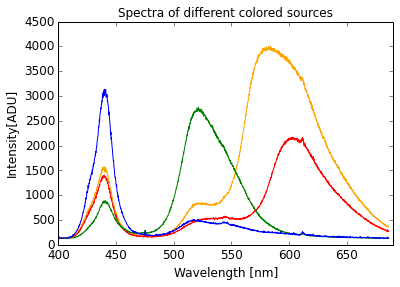
\includegraphics[width=0.5\textwidth]{figures/color}
\caption{ Each colored line shows the spectral response to the corresponding color filters. The difference in relative intensity is irrelevant, it is may simply be due to how close we are holding the source to the entrance slit of the spectrometer and how efficient the colored-marker ink is at blocking out light. Pixel-to-wavelength conversion done by manufacturer's wavelength calibration coefficients.}
\label{color}
\end{figure}
	\paragraph*{\textbf{Voltage}} The desk lamp is attached to an external potentiometer which allows us to vary the voltage of the source. Since to the relationship between voltage and current is described by Ohm's law, the decrease in voltage is directly proportional to the decrease in current, which  leads to a dimming of the lamp. Another way is to consider the power dissipation by the bulb as described by Eq. \ref{power_ohms}
	\begin{equation}
	P=IV=\frac{V^2}{R}
	\label{power_ohms}
	\end{equation}
		where P is the power dissipated by the lamp, I is current through the lamp, V is the voltage across the circuit (externally modulated by the potentiometer) and R is the resistance of the circuit which in this case is fixed. Therefore, decreasing the voltage also cause a decreases in power dissipation.
		
If we approximate the desklamp source as a radiating blackbody, Wien's law states that its wavelength distribution for different temperature should be approximately the same shape but with a displaced wavelength as shown in Eq.\ref{wien}:
		\begin{equation}
		\lambda_{max} = \frac{b}{T}=\frac{2.897\times 10^3 m\cdot K}{T}
		\label{wien}
		\end{equation}
		where $\lambda_{max}$ is the peak wavelength for the distribution, T is the temperature of the radiating blackbody, and b is the Wien's displacement constant.
		Since Eq. \ref{power_ohms} shows a lower power dissspation for smaller input voltage, it means that the lamp's bulb is cooler in temperature than if it was at a higher voltage setting. This is why the peak wavelength of the  lower-voltage source distribution is longer than the higher-voltage source. % hy the spectra taken with the low voltage setting peaks at a lower wavelength is
	\begin{figure}[h!]
	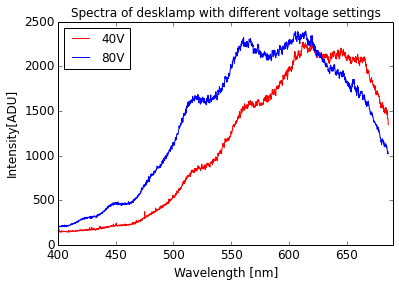
\includegraphics[width=0.5\textwidth]{figures/voltage}
\caption{Changing the input voltage of the source affects the peak wavelength of the distribution. }
\label{voltage}
	\end{figure}
\subsection{Spectra property and comparison for different sources}
\section{Systematic Effects}
	 \subsection{Natural Broadening Effect}
 As seen in Fig. (LABEL HERE) the spectral lines do not resemble perfectly sharp Dirac Delta functions. This broadening effect is due to several physical phenomena, one reason is the natural line width caused by the measurement uncertainty inherent from quantum mechanics. Another more dominant effect is due to Doppler shift from the thermal velocity of the atoms. The distribution of the atomic thermal velocity is governed by the Boltzmann distribution. This Doppler-shifted velocity distribution propagates to our intensity measurement, which can then be rearranged into a Gaussian form. The broadening effect is characterized by the variance of this new distribution as shown in  Eq. \ref{doppler_var},
 \begin{equation}\label{doppler_var}
\sigma_f = \sqrt{\frac{kT}{mc^2}}f_0
 \end{equation}
 where T is the temperature, m is the mass of the atom, $f_0$ is the frequency when atom is stationary, c is the speed of light and k is the Boltzman factor.
 

Possible source of error: 
- ununiform pixels(REF dark counts)
- multiple mixed source since roomlight not closed when taking data, so slight traces of other sources in our pure data like neon...etc
\section{Read Noise and gain}
We chose to conduct the statistical analysis on noise property on the 60Watt lightbulb data since the variance is less likely to be dominated by fluctuations in the source's illumination brightness compared to the sunlight or plasma bulb.
 \subsection{Dark Counts}
 We took set of 3ms integration time bias frames by placing the red cap on the spectrometer and in a black bag. This integration time was chosen as close to zero as possible to minimize the tails of the Gaussian on the two ends. The 3ms integration time is the shortest integration time accessible for data acquisition using the SpectraSuite software. 
 %A histogram of dark counts is fitted to a Gaussian. 
 %The variance of the distribution relates to the read noise and gain of the spectrometer \citep{ccd_handbook}. 
 
A Gaussian is fitted onto the histogram to obtain the value of mean ($\mu$) and variance($\sigma$) of the distribution. The $\mu$ corresponds to the $ADU_0$, whereas the $\sigma$ corresponds to $\sigma_{ADU_0}$, the error on the dark counts. This variation on the dark counts comes from the non-uniform quality of the pixel as seen in Fig.\ref{dark_counts}. But since $\sigma_{ADU_0}$ is relatively small compared to $ADU_0$, it is negligible when considering its per-pixel additive effect on the raw data.


In real astronomical observations, this method of acquiring dark measurements and the use of overscan strips by adding additional pseudopixels are two common ways of bias calibration on imaging data. Although our spectrometer has a linear CCD array as a detector, imaging telescope often has an plane array of CCD pixels. In those cases, an average of 10 or more bias frame is often better bias-correction technique since it reveals any underlying 2D bias patterns present. 
 \begin{figure}[h!]
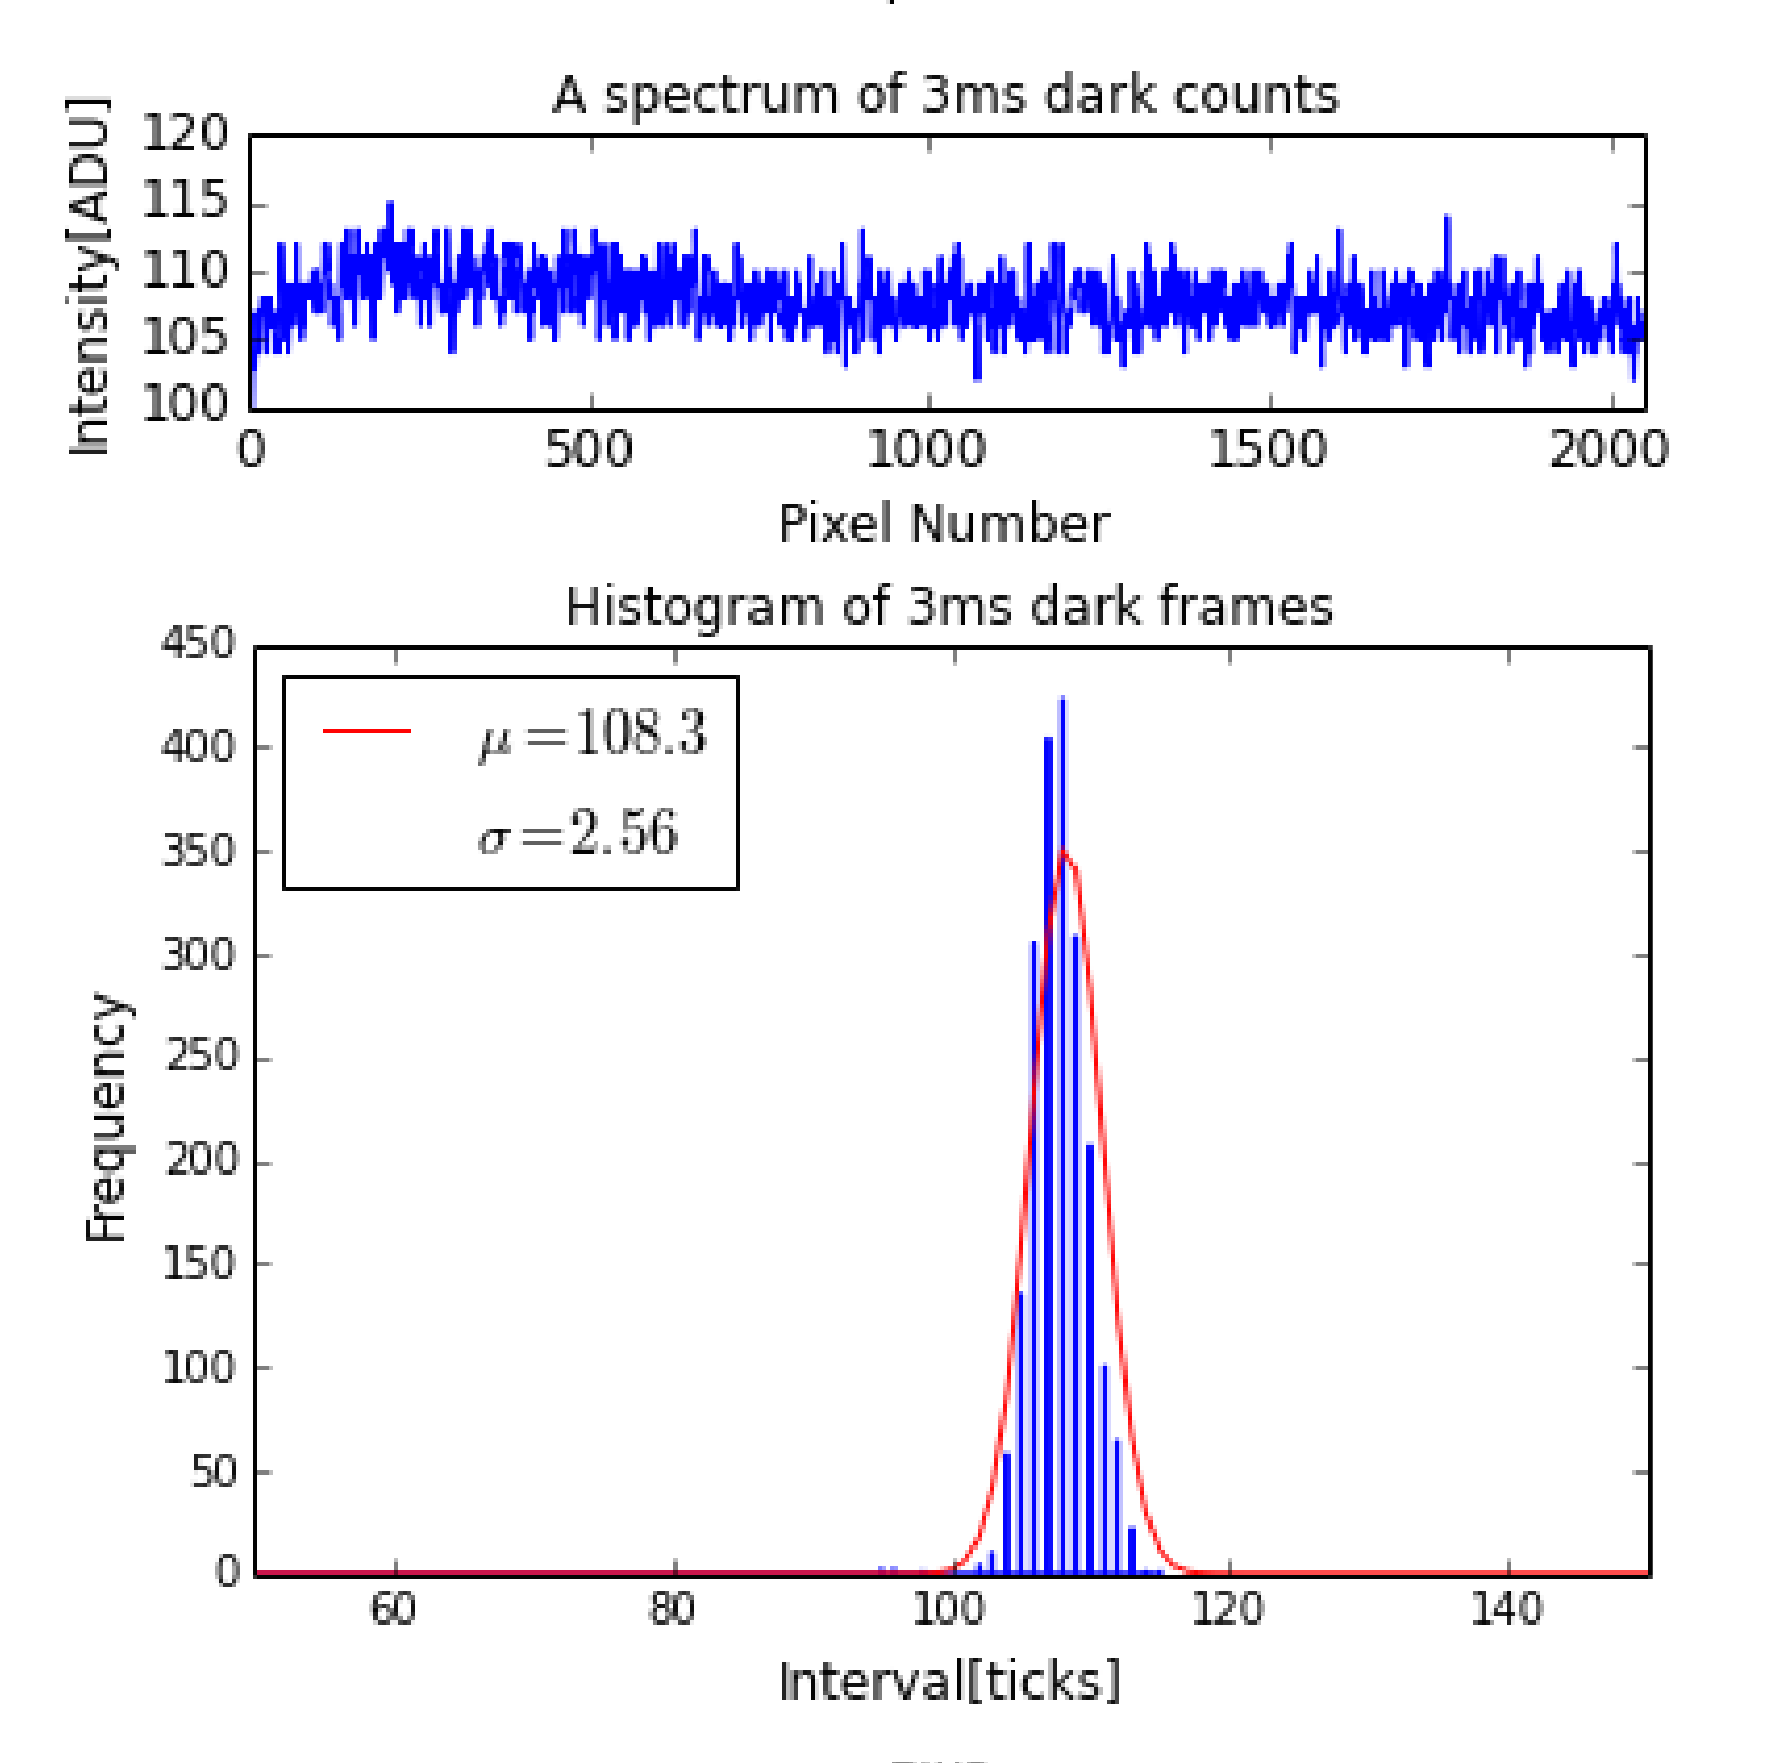
\includegraphics[width=0.45\textwidth]{figures/dark&biashisto}
\caption{Top panel shows an averaged spectra of dark counts that exhibits the non-uniformity of each pixel in the linear CCD array. Also, note the clear bias offset seen at around 125 ADU. Bottom panel is a histogram of bias frames fitted with a Gaussian. } 
\label{dark_counts}
\end{figure}
\section{Data Reduction}
 Now we have examined the systematic effects that affects our data, we process the raw data obtained from the spectrometer in order to find an equation that converts the pixel values to wavelengths.
  \subsection{Data Smoothing}
  Smoothing is a data reduction technique that removes noise and minor pixel-to-pixel variations in the data. We employ both the boxcar and averaging technique in our datasets and compare their resulting differences.
  \paragraph*{\textbf{Boxcar Smoothing}}
  Our boxcar smoothing algorithm takes the values of adjacent pixel and average them over some user-defined interval. Since the quality of each pixel is inconsistent, boxcar smoothing compensate for 
  However even though boxcar smoothing lowers the signal-to-noise ratio by eliminating small-scale features, when 
  boxcar smoothing may lower the resolution of the Delta-function-like peak that  important spectral fec
  In this case could be useful for better centroid findindg 
Since the quality of each pixel is inconsistent, we employ boxcar smoothing to compensate for the 



  
   boxcar average for cosmetic purposes. lower s/N but resolution decrease. 
   
This produced undesirable results so we resorted to the conventional averaging of data by averaging over whole datasets
  a step towards finding a functional form to fit the data  into functional form since it makes the data less discrete and more continuous like a function.l

	\subsection{Automated centroid algorithm}
	We attempted to create an automated centroid algorithm by imposing two conditions to select for the centroid of interest that correspond to atomic signature spectral lines. The selected data range used for centroid calculation must begin at a local minimum and contain one local maximum and then end with another local minimum. There can not be any extra extrema that lies within that range other than the 3 specified. Since a large number of datapoints satisfies this condition, we needed a quantitative measure of how ``important" the spike is.  For this, we use the intensity difference between the consecutive  local maximum and minimum and select only the data ranges that  have  differences greater than 10\% of the difference between the absolute maximum and  minimum datapoint of the whole dataset. The ad hoc 10\% criterium was chosen to so that the bias offset  was considered in . The 10\% was chosen because of the quality of the centroid result that it produces. The local extrema was found by comparing consecutive data points and testing a change in the boolean condition of increasing or decreasing.
\begin{figure}
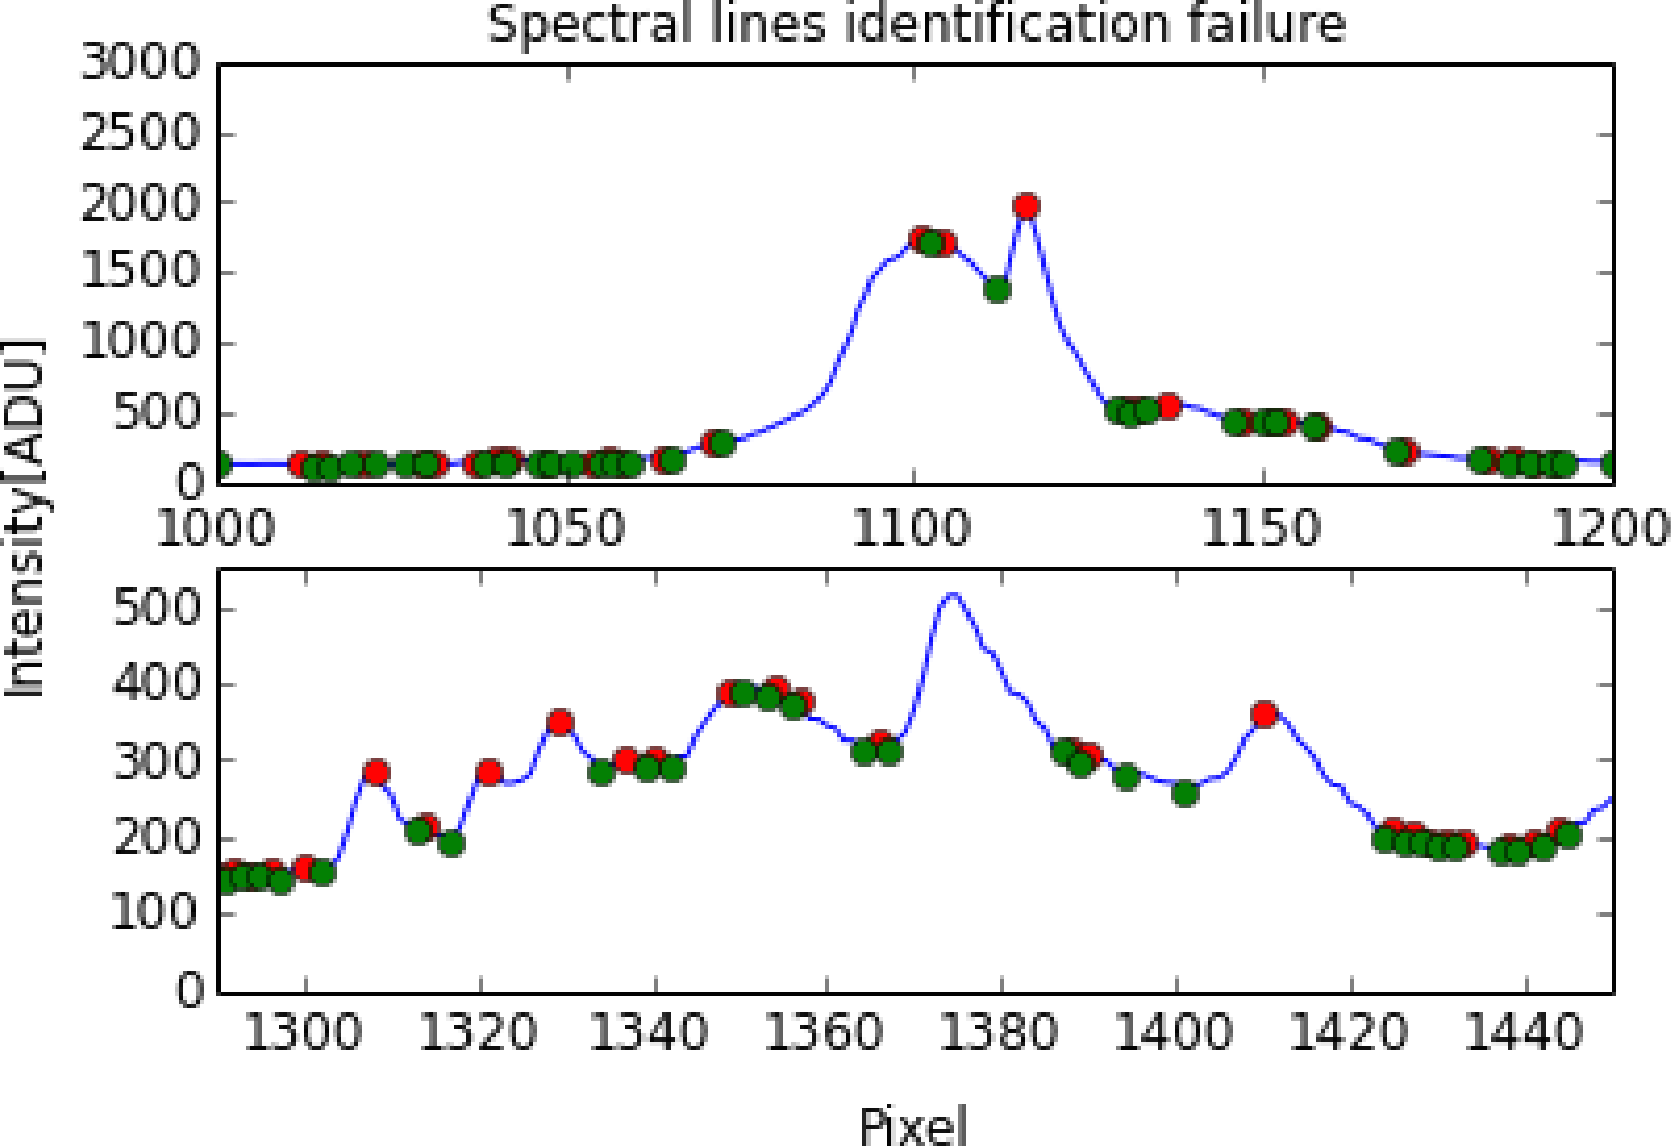
\includegraphics[width=0.45\textwidth]{figures/fail}
\caption{Top: The closely spaced extremum at around the 1100th pixel results in a small difference value between the local minimum and maximum. Therefore, it was not detected by the algorithm. Bottom: The extremum finding algorithm did not detect the maximum at around pixel 1380 in its  first step.}
\end{figure}
	%the algorithm is robust as it is proven to find accurate centroid on a test data of 10000 sample (do later)
	The alogirthim was not very robust as it is unable pick out spectral lines that lied between consecutive extremas such as the ones on pixel 1115 and 1374. Despite varying the percentage cut, it was unable to identify features that showed relative difference such as 314 but only measured the absolute differences, which is hard to account for with such great differences.
\begin{figure}
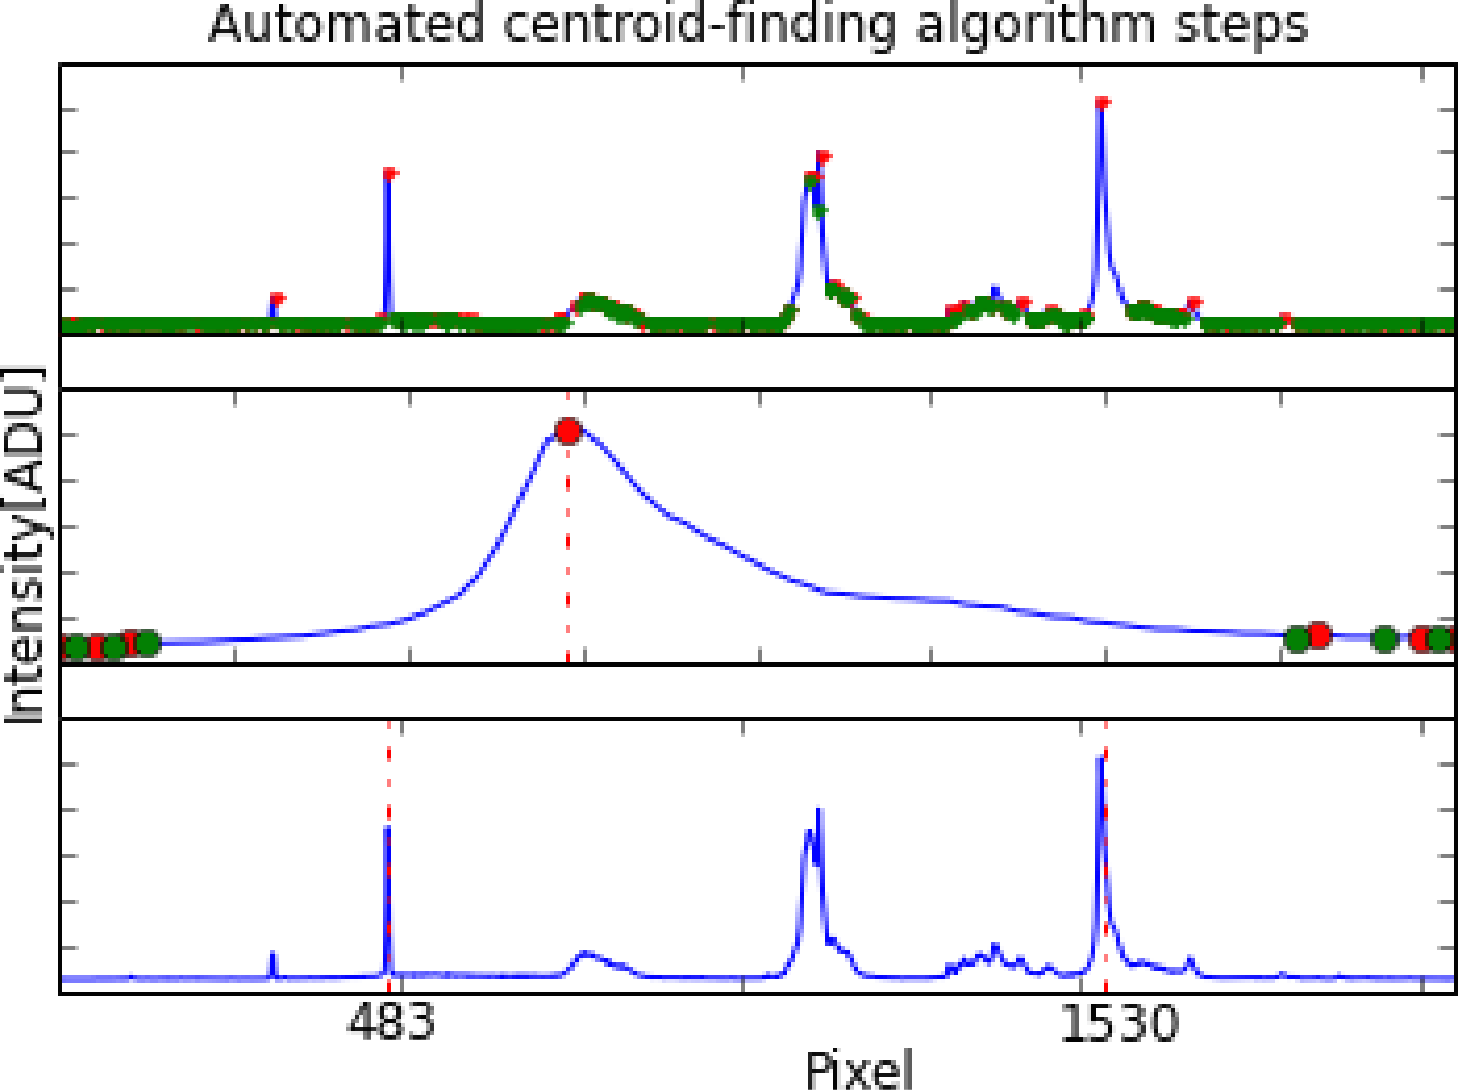
\includegraphics[width=0.45\textwidth]{figures/steps}
\caption{Graphical representation of how the automated algorithm works. Top: Identifying all the extremum of the dataset. Red marker denotes local maximum; green denotes local minimum. Middle: Applying criteria to select suitable ranges as shown in middle plot, using this sliced dataset to obtain the centroid values (dashed). Bottom: Resulting centroid list misses some important spectral feature picked out by the eyeball-estimation method shown in Fig. (\textbf{REF!!!!}).} 
\end{figure}
\subsection{Wavelength calibration}
The polynomial nature of our fitting model comes from the paraxial apprximation of diffraction scneario, which results in a Taylor expansion that can be boiled down to a polynomial of higher order terms.
\begin{figure}
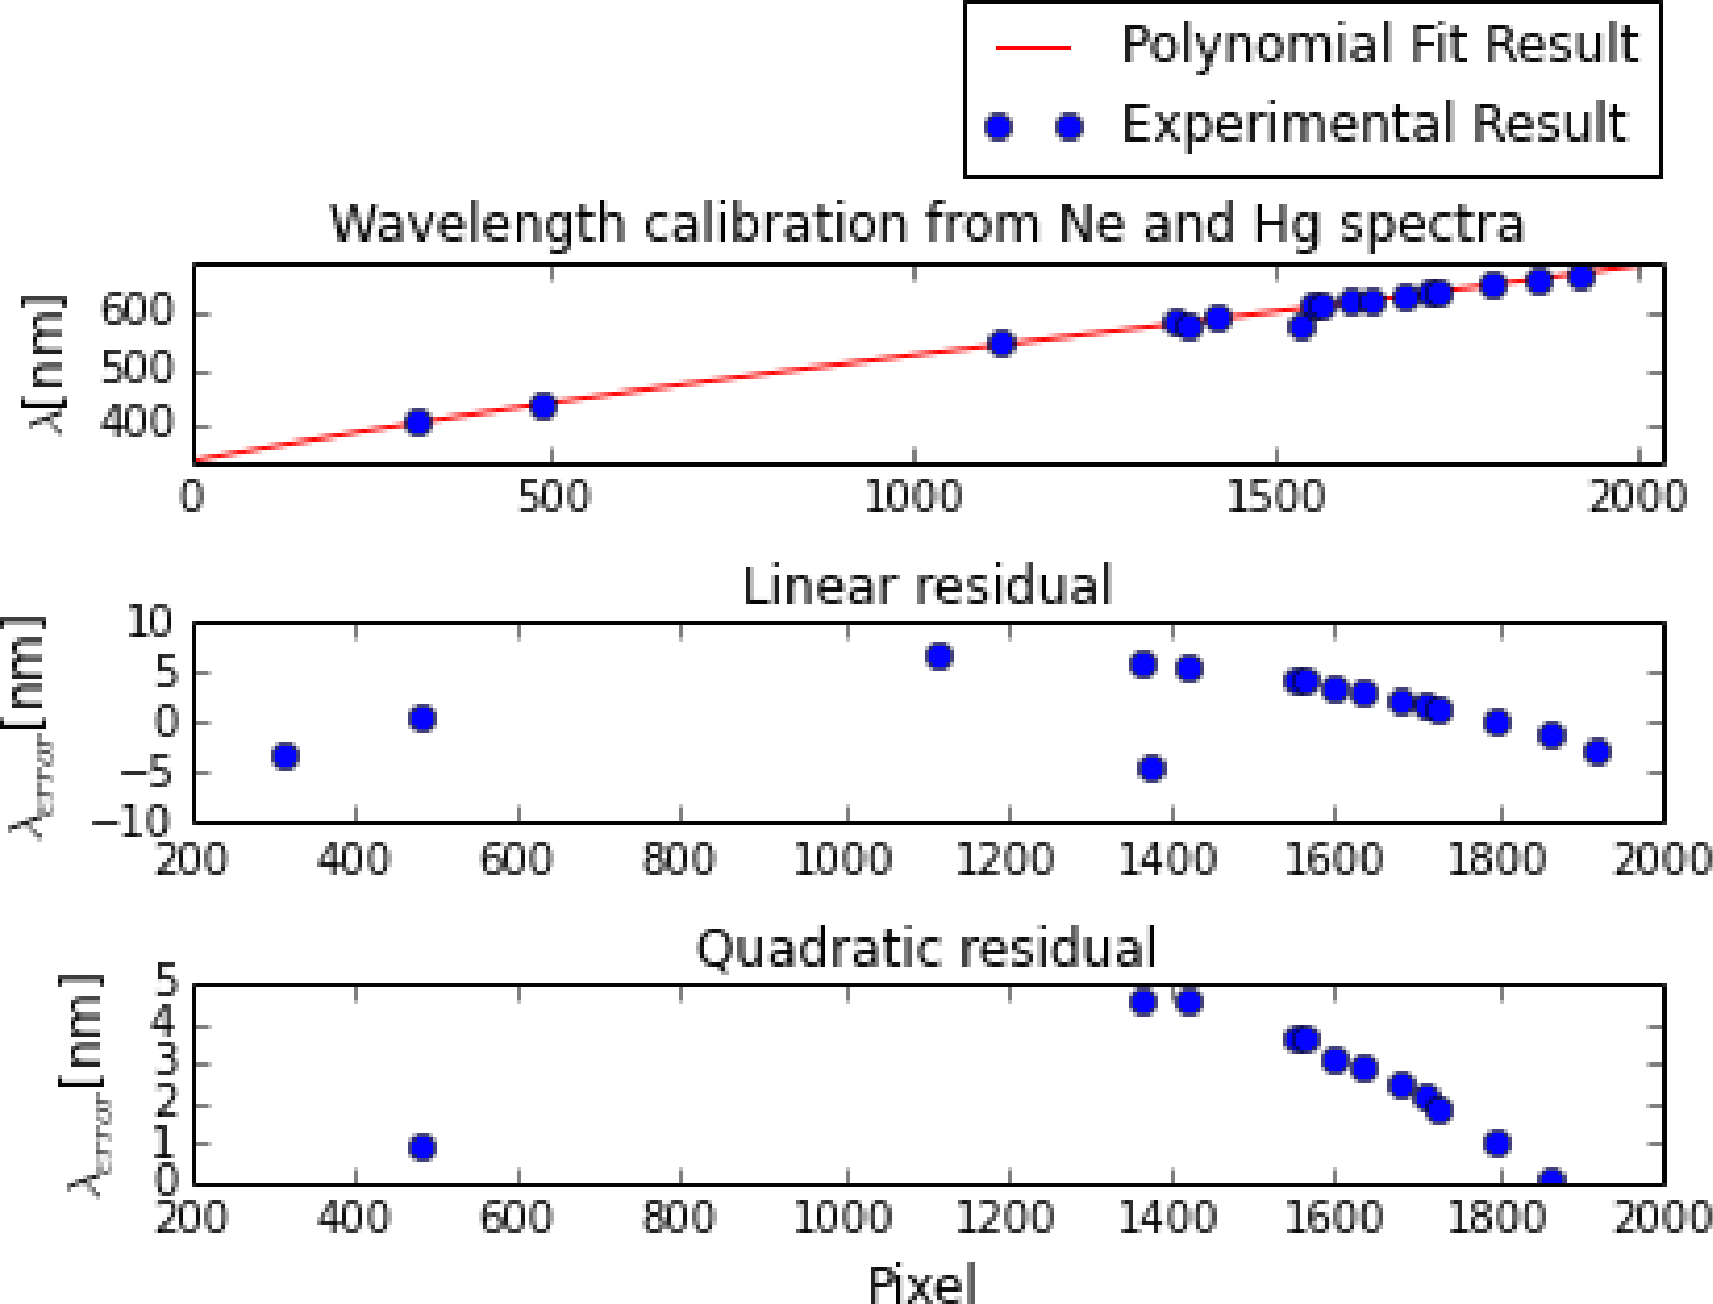
\includegraphics[width=0.5\textwidth]{figures/neon_calib}
\caption{ } 
\end{figure}
\section{Conclusion}
Possible extension to this project may be to try conducting a basic flat-field correction to the detector. One way to do this to shine bright light uniformly on the detector to see the response of each pixel. The exposure time needs to be short so that the CCD is not saturated. We can also try to measure maximum ranges at which CCD is sensitive and linear.
\bibliography{references}
 %\bibliographystyle{abbrvnat}
%\bibliographystyle{apalike}
%\bibliographystyle{plainnat}
%\bibliographystyle{unsrtnat}
\bibliographystyle{elsarticle-harv}
Haken, Hermann and Wolf, Hans Christolph, The Physics of Atoms and Quanta, 5th Ed., Springer-Verlag, 1996.
\end{document}
